
\documentclass[a4paper]{article}

\usepackage[ngerman]{babel}
\usepackage[utf8]{inputenc}
\usepackage{longtable}
\usepackage{graphicx}
\usepackage{graphics}
\usepackage[pdfborder={0 0 0}]{hyperref}
\usepackage{geometry}
\usepackage{float}
\usepackage{fancyhdr}
\usepackage{titling}
\usepackage{csquotes}
\usepackage{minted}
\usepackage{xcolor}
\usepackage{verbatimbox}
\usepackage{textcomp}

\newcommand{\subtitle}[1]{%
  \posttitle{%
    \par\end{center}
    \begin{center}\large#1\end{center}
    \vskip0.5em}%
}

\newenvironment{fullgrayverb}
{\verbbox}
{\endverbbox\par\colorbox{lightgray}{\parbox{\textwidth}{\theverbbox}}\par}

\title{Netzwerk- und System-Management-Projekt}
\subtitle{Netzwerk- und Service-Struktur einer Fakultät}
\date{\today}
\author{Tom Wegener, 18INM/TZ}


\geometry{a4paper, left=30mm, right=20mm,top=25mm,bottom=25mm}
  \fancyhead{}
  \fancyhead[L]{Tom Wegener, 18INM/TZ}
  \fancyhead[R]{Abschlussbericht NSM}
  \fancyfoot{}
  \fancyfoot[R]{\thepage}

\setlength{\parindent}{0em}


\begin{document}

\pagestyle{empty}

\maketitle

\newpage

\tableofcontents

\newpage

\pagestyle{fancy}

\setcounter{page}{1}

\section{Einleitung}
Für das Modul Netzwerk- und System-Management (NSM) sollen die Studierenden des Studiengangs "Informatik Master" der HTWK Leipzig die Infrastruktur einer Fakultät erstellen, die sich außerhalb des Universitäts-netzes befindet.

Das Projekt soll mit Hilfe von Netkit als virtuelle Infrastruktur realisiert werden und anschließend über Ansible konfiguriert werden.

\subsection{Umgebung}

Das Projekt wurde nicht innerhalb der VM umgesetzt, sondern für bessere Performance direkt auf einem privaten Rechner umgesetzt. Auf dem Rechner ist eine Linux-Distribution, die auf Ubuntu 18.10 basiert, installiert. Dabei hat Ansible die Version 2.7.8 und nutzt die Python-Version 3.6.7. Anstatt der originalen Netkit-Version wurde \href{https://netkit-ng.github.io/}{Netkit-ng} genutzt, welches ein neueres Filesystem nutzt, das auf Debian wheezy basiert.
Die Verbindung zwischen dem host und den Netkit-VMs wird über SSH realisiert in einer Agent-less Architektur.

Durch die trotzdem veraltete Version des Netkit-File-Systems können einige Sachen nicht wie im Konzept beschrieben umgesetzt werden. Durch ein Update des File-Systems auf eine neuere Debian-Version, kann dies ermöglicht werden. Für dieses Projekt wurde versucht, die bereits vorhandene Software so wenig wie möglich zu verändern. Dementsprechend sind auch nur relevante Applikationen auf den VMs aktuell, es wurde kein generelles Update ausgeführt.

\newpage

\section{Konzept}
Es soll die Infrastruktur einer externen Fakultät realsiert werden.

\subsection{Anforderungen}
Das Netzwerk der Fakultät erhält Internet und Anbindung an die Universität über eine sogenannte Dark Fiber-Leitung, diese ist eine bisher ungenutzte und angemietet Leitung eines bereits verlegten Netzes. Des Weiteren werden durch die Fakultät Services, wie Mail, ein Web-Auftritt und AAA-Services angeboten.

\subsection{Konzeption}
Die Infrastruktur besteht grundlegend aus drei Subnetzen, sowie einem großen Netzwerk. Die Verbindung der Subnetze wird über das Kern-Netzwerk bzw. den Kern-Router ermöglicht. Zusätzlich zu dem Kern-Router hat jedes Subnetzwerk einen Router und der Anschluss über die Dark-Fiber-Leitung wird auch über einen Router realisiert. Die drei Subnetzwerke sind die demilitarisierte Zone (DMZ), das Server-Netzwerk und das Client-Netzwerk. Das Netzwerk ist in der Abbildung \ref{fig:model} grafisch dargestellt.

\begin{figure}[H]
  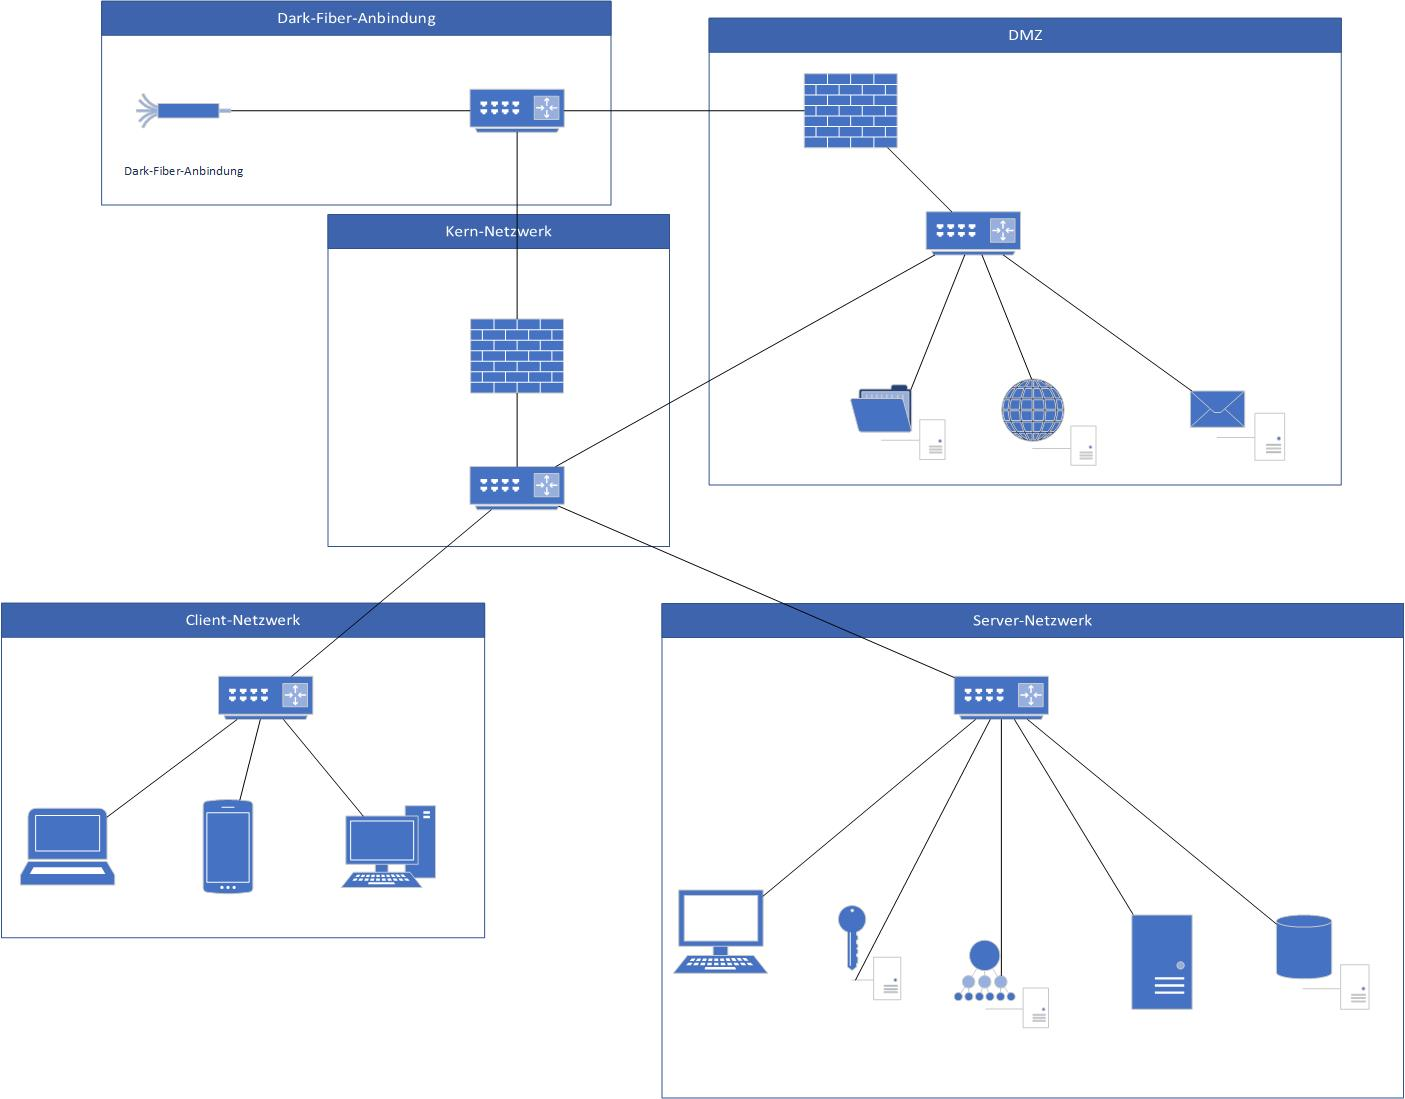
\includegraphics[width=\linewidth]{pictures/netzwerk-diagramm.jpg}
  \caption{Modell der Infrastruktur}
  \label{fig:model}
\end{figure}

In der Abbildung ist pro Netzwerk nur ein Router eingezeichnet, um die Übersichtlichkeit zu verbessern. Es sollte bei einer Umsetzung bedacht werden, dass es mindestens zwei gibt, um einerseits einen Ersatz bei einem Ausfall zu haben, aber auch, um  ein Load-Balancing zu ermöglichen.

Die DMZ stellt alle Dienste bereit, die über das Internet erreichbar sein sollen, also einen Web-Server, einen Mail-Server und einen AAA-Server. Jedoch werden kritische Daten nicht auf Servern in der DMZ gespeichert, sondern sind auf Servern in dem Server-Netzwerk gespeichert, die jedoch über Server aus der DMZ erreichbar sind.

Das Server-Netzwerk ist für die Bereitstellung von Daten und Diensten innerhalb der Fakultät zuständig. Zur Sicherheit sollten keine Daten aus diesem Subnetz direkt den Dark-Fiber-Router passieren, sondern maximal über einen Server der DMZ abgefragt werden und dann weitergeleitet werden. Eine Ausnahme bilden Programme, die auf den Servern benötigt werden.

Die Rechner der Angestellten der Fakultät, sowie der Studierenden der Fakultät, sind alle im Client-Netzwerk. Die Administration erfolgt ebenfalls über einen Rechner im Client-Netz.

Generell soll das Netzwerk durch das Tool \href{www.theforeman.org}{Foreman} gemanaged werden. Foreman ermöglicht die Administration von Hosts und kann auch für die Administration von großen Netzwerken samt Routern, Clients und Servern genutzt werden. Über eine grafische Web-Oberfläche wird es ermöglicht einen Überblick zu behalten, sowie die Provisionierung und die Konfiguration abzuwickeln.
Das Administrationstool wickelt die Konfiguration eigentlich über Puppet ab, kann jedoch durch Plugins erweitert werden, wie dem Ansible-Plugin. 

Außerdem kann Foreman auch bei der Realisierung von FCAPS helfen.

\subsection{FCAPS}
FCAPS ist ein Modell für das Management von Netzwerken bzw. Infrastrukturen, es ist ein Akronym für Fault-Management, Configuration-Management, Administration and Accounting Management, Performance Management und Security Management. FCAPS wird in diesem Fall über verschiedene Tools realisiert.


\subsubsection{Fault-Management}
Fault-Management bedeutet das frühzeitige Erkennen und Beheben von Fehlern innerhalb des Netzwerkes, das kann durch z.B. eine Icinga-Instanz realisiert werden. Alternativ kann auch ein anderes Werkzeug, wie z.B. Foreman, genutzt werden, welches mehrere Teile von FCAPS in sich vereinigt.

Foreman überprüft die Anwesenheit und Funktionalität von Hosts durch puppet-nodes, außerdem kann durch ein Plugin zentralisiertes Logging umgesetzt werden. Sollte ein Fehler auftreten, der unter eine bestimmte Einstufung, wie z.B. ''kritisch'' fällt, kann eine Benachrichtigung gesendet werden, außerdem wird auch ein vereinfachtes Handeln unterstützt, solange eine Verbindung zum Host besteht, können Logs abgerufen werden, Konfigurationen erneut angewendet werden oder Updates gefahren werden.

Für ein übersichtliches Logging müssen die Logs in verschiedene Stufen eingeteilt werden. Es empfiehlt sich, diese einerseits nach Gefahr für die weitere Funktionalität einzuteilen, wie auch in die verschiedene Komponenten. So können Logs, wie ''critical: infrastructure: lost connection to mail-server'' schnell verstanden werden.

\subsubsection{Configuration Management}
Das Konfigurationsmanagement wird über Ansible abgewicklet. Dabei werden die einzelnen benötigten Dienste als Konfigurationen in playbooks angelegt, die einen entsprechenden Namen haben, sollte ein Host ausfallen, kann in der host-Datei ein neuer Host der entsprechenden Gruppe hinzugefügt werden. Theoretisch können die Konfigurationen der Router ebenfalls über playbooks abgespeichert werden. 

Durch eine Integration von Ansible in Foreman über das dazugehörige Plugin kann die Ausführung von playbooks einfach umgesetzt werden, sowie die Ausführung überwacht werden. Die Ergebnisse der Ausführung werden bei Foreman je Host aufgelistet.

\subsubsection{Administration and Accounting Management}

\subsubsection{Performance Management}
Performance Management bedeutet die Überwachung der Performance aller Komponenten des Netzwerkes. Dabei muss die Auslastung der Server, die Gesundheit und das Alter von Festplatten und anderen (Netzwerk-)Komponenten überwacht werden.

\subsubsection{Security Management}
Security Management bedeutet sich über die Sicherheit der Infrastruktur bewusst zu sein und diese so gut wie möglich zu verbessern. Das beinhaltet die physische, sowie die digitale Sicherheit.

Die physische Sicherheit wird unter Anderem durch eine Zugangskontrolle zu den Räumen in denen die Server stehen erreicht. Jedoch werden noch weitere Schritte benötigt.

Die digitale Sicherheit kann unter Anderem durch IPSec realisiert werden, außerdem muss ein Überblick über wichtige Sicherheits-Updates beibehalten werden und diese durch das Konfigurations-Management aufgespielt werden.

Die Authorisierung für die Dienste und das Netzwerk wird über den AAA-Server realisiert.

Alle über das Internet erreichbaren Dienste können nur über https erreicht werden, während bestimmte Dienste, wie ein File-Server, nur über ein VPN erreichbar sind.

Außerdem wird der Zugriff auf z.B. das Server-Netzwerk aus dem Internet eingeschränkt. Die es kann nur aus dem Client-Netzwerk und der DMZ auf Daten, die auf diesen Servern liegen zugegriffen werden. Außerdem werden über die beiden Firewalls die Zugriffe zusätzlich beschränkt und verschiedenen IP-Adressen geblockt.

\section{Umsetzung}

Für die Umsetzung musste statt dem originalen Netkit Netkit-ng genutzt werden, welches python2.7 unterstützt, das für Ansible benötigt wird. Ein Update der Netkit-Instanzen auf python2.7 war auf Grund des Alters nicht möglich.

Es wurde eine wie in \ref{fig:model} Topologie erzeugt und über statische Routen eine grundlegende Netzwerk-Kommunikation ermöglicht. Über die VM ''darkfiber-r'' wird eine Internet-Anbindung realisiert, wie sie in den Anforderungen gefordert wird.
\subsection{Ausblick}

\section{Fazit}

\newpage

\section{Anhang}
\subsection{Glossar}

\begin{fullgrayverb}
>ref|XP_021694431.1| gametogenetin-binding protein 2-like [Aedes aegypti]
MAKLTYVYRSDEMNCVKVSKRQLPLIGGENLMMLMDLNSRGLVFDQPPVKGQELDDFAKKYRVLTPAELR
LSLNVPTIEFTSVLSQNVPCVGCRRSVERLFYQLMLSGHPTLDPIVITGRGVLTISEDKMKSPQ...
\end{fullgrayverb}\\


\end{document}
